\chapter{Seguridad en redes}

En el presente tema, dejaremos por un momento de lado la capa de transporte para centrarnos en la seguridad en las comunicaciones, concepto esencial que iremos detallando a lo largo de las siguientes páginas.

\subsubsection{Objetivos}
\begin{itemize}
    \item Comprender la importancia de la seguridad en las comunicaciones y aprender cómo desplegar mecanismos básicos de seguridad en redes de computadores e Internet.
    \item Conocer los aspectos de seguridad en redes: confidencialidad, autentificación, no repudio, integridad y disponibilidad. 
    \item Entender los conceptos básicos de la seguridad en redes, como el uso de algoritmos de clave secreta, de clave pública, intercambio de claves\ldots
    \item Comprender qué son los certificados digitales y las autoridades de certificación, y los diferentes mecanismos que se pueden implementar con certificados. 
    \item Conocer algunos de los principales protocolos de comunicación seguros, como \acrshort{TLS} e \acrshort{IPSec}, y los mecanismos que lo utilizan. 
\end{itemize}


\section{Introducción}
Una red de comunicaciones es \textbf{segura} cuando se garantizan todos los aspectos de seguridad, por lo que no hay protocolos ni redes 100\% seguras. No obstante, el objetivo de una red debe ser cubrir todos los aspectos de seguridad posibles.
Definamos brevemente los aspectos de seguridad que vamos a estudiar, junto con los métodos que se utilizan para garantizarlos.
\begin{itemize}
    \item \textbf{Confidencialidad / privacidad:} se garantiza que, cuando transmitimos algo a un receptor determinado, tan solo dicho receptor sea capaz de ver el mensaje.\\
    Se consigue con el cifrado. 
    \item \textbf{Autenticación:} las entidades son quien dicen ser.\\
    Se consigue con algoritmos de Reto-Respuesta o doble cifrado. 
    \item \textbf{No repudio o irrenunciabilidad:} 
    no se permite la renuncia de la autoría de determinada acción, por lo que se convierte en una prueba legal en ante un juez en el caso de ser necesario. Por ejemplo, no podemos renunciar haber participado en una transacción.\\
    Se consigue con la firma digital o con el doble cifrado con certificado, pero ha de haber una entidad fiable. 
    \item \textbf{Integridad:} se garantiza que los datos no sean manipulados por el camino (intencionadamente o no).\\
    Se consigue con funciones hash o compendios (resúmenes).
    \item \textbf{Disponibilidad:} el sistema mantiene las prestaciones de los servicios independientemente de la demanda\footnote{Este aspecto no se tratará en la asignatura.}.
\end{itemize}

Como hemos mencionado antes, una red es \textbf{segura} cuando se garantizan todos los aspectos de seguridad, y esta debe estar presente en todos los niveles de la red. El grado de seguridad lo \emph{fija el punto más débil}, ya que este es el punto más vulnerable y por el que se podría producir un ataque de seguridad. Por tanto, es importante que haya seguridad en todos los niveles de la red.

\begin{definicion}[Ataque de seguridad]
    Cualquier acción intencionada o no que menoscaba cualquiera de los aspectos de seguridad. 
\end{definicion}

Veamos algunos ejemplos de ataque de seguridad:
\begin{itemize}
    \item \textbf{Sniffing:} escuchar comunicaciones, por ejemplo mediante Wireshark. Se produce una vulneración de la confidencialidad.
    \item \textbf{Snooping (phishing):} suplantación de la identidad de alguna entidad. Se vulnera la autentificación.
    \item \textbf{Man in the Middle:} un atacante se situa en medio de dos equipos que se comunican e intercepta todos los mensajes que se transmiten.
    \item \textbf{\acrfull{DDoS}:} ataque consistente en enviar muchas peticiones a un servidor para que este no pueda atender a todas, consiguiendo que el servicio deje de funcionar. Se denomina \emph{distributed} si las peticiones provienen de distintos equipos, que suele ser lo más común. 
    \item \textbf{Malware:} software malicioso, como troyanos, gusanos, \textit{spyware}, \textit{backdoors}, \textit{rootkits}, \textit{keyloggers}, etc. Un ejemplo es \textit{ransomware}, en el que se encriptan todos o parte de los datos y se pide un recate a cambio de estos.
\end{itemize}


Los mecanismos de seguridad que vamos a estudiar, como hemos mencionado antes, son:
\begin{itemize}
    \item Para garantizar la confidencialidad:
    \begin{itemize}
        \item Cifrado (simétrico y asimétrico).
    \end{itemize}
    \item Para garantizar la autentificación:
    \begin{itemize}
        \item Autentificación con clave secreta (reto-respuesta).
        \item Intercambio de Diffie-Hellman (establecimiento de clave secreta).
    \end{itemize}

    \item Para garantizar la integridad:
    \begin{itemize}
        \item Funciones Hash (\acrfull{HMAC}).
    \end{itemize}

    \item Para garantizar el no repudio:
    \begin{itemize}
        \item Firma digital.
        \item Certificados digitales.
    \end{itemize}
\end{itemize}

\section{Cifrado}
Se trata de un procedimiento para garantizar la confidencialidad.\\


El proceso se ilustra en la Figura~\ref{fig:cifrado/descifrado}. Inicialmente, se dispone de un texto plano a transmitir (P), que buscamos que tan solo pueda ser leído por el receptor. Para ello, se emplea una función de cifrado $E_k$ que dará lugar a un texto cifrado (C), el cual se mandará a través del canal de comunicaciones (no supone un problema, ya que este texto cifrado no será entendible). Llegará al otro extremo y será descifrado con una función $D_{k'}$, obteniendo así de nuevo el texto plano (P).

Los algoritmos de cifrado y descifrado ($E_k$ y $D_{k'}$) normalmente son conocidos, pero estos dependen de claves $k$ y $k'$ que son secretas. La dificultad reside en hallar estas claves.
\begin{figure}[H]
    \centering
    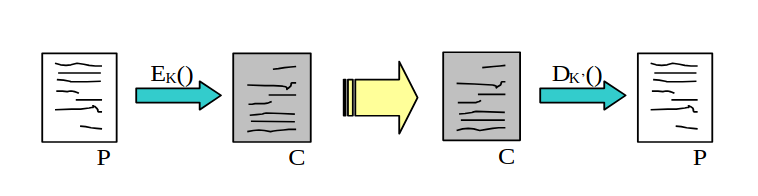
\includegraphics[width=1\linewidth]{./images/cifrado.png}
    \caption{Proceso de cifrado y descifrado.}
    \label{fig:cifrado/descifrado}
\end{figure}

Veremos dos tipos de algoritmos de cifrado:
\begin{itemize}
    \item Cifrado simétrico. La clave es secreta y única ($k=k'$), y se usan distintas funciones para cifrar y descifrar.
    \item Cifrado asimétrico. Hay dos claves (pública y privada), y se usa la misma función para cifrar y descifrar.
\end{itemize}

\subsection{Cifrado simétrico}

Este tipo de algoritmos de cifrado se denomina simétrico porque se usa la misma clave para cifrar y descifrar los datos. Por tanto, la clave es secreta y tan solo es conocida por el emisor de los datos y el receptor.

\subsubsection{\acrfull{DES}}
Se trata de algoritmo de cifrado simétrico que se basa en realizar permutaciones y funciones \verb|XOR| encadenadas. Se cifran palabras de 64 bits usando para ello una clave de 56 bits.

Como principal ventaja, como estas operaciones se pueden implementar de forma sencilla en hardware, es un algoritmo muy rápido, por lo que se puede usar en tiempo real (por ejemplo para codificar voz). 

No obstante, presenta una serie de problemas:
\begin{itemize}
    \item La longitud de la clave es corta ($2^{56}$ posibles claves), por lo que es vulnerable a ataques de fuerza bruta.
    \item Lo que se termina obteniendo es una sustitución, por lo que con la misma entrada el resultado siempre será el mismo. Usando estudios estadísticos dependiendo del idioma, se puede llegar a descifrar el mensaje.
\end{itemize}

Para mitigar este segundo aspecto, se utiliza un esquema de cifrado reentrante, donde la salida de aplicar una transformación se usa para el cifrado de la siguiente palabra a cifrar. De esta forma, quien recibe el mensaje codificado necesita conocer la última entrada usada para codificar y podrá así aplicar el proceso inverso.

\subsubsection{DES doble y 3DES\@}
Son mejoras de DES que proporcionan robustez al algoritmo. Se toman dos claves $k_1$ y $k_2$ y para cifrar se toma una función $E$ y su inversa $D$ y se concatenan $E_{k_1}$, $D_{k_2}$, $E_{k_1}$ y para descifrar se concatenan $D_{k_1}$, $E_{k_2}$, $D_{k_1}$. 
\subsubsection{IDEA\@}
Usa la misma idea que DES pero con claves de 128 bits, lo que aumenta la complejidad de violación del protocolo. 

\subsection{Cifrado asimétrico}
Cada usuario $A$ tiene una clave pública $K_{pub_A}$ y una clave privada $K_{pri_A}$ distintas. Conociendo la pública no es posible conocer la privada, por lo que la pública la conocen todos pero la privada solo la conoce $A$. 
\begin{equation*}
    C = K_{pub_A}(P) \rightarrow P = K_{pri_A}(C)
\end{equation*}
\begin{equation*}
    C = K_{pri_A}(P) \rightarrow P = K_{pub_A}(C)
\end{equation*}

Esta es la forma de funcionar de cualquier cifrado con clave pública. Además hay una correspondencia biunívoca entre las claves públicas y privadas. 
\subsubsection{RSA\@}
\noindent
Es un algoritmo para sacar las claves del cifrado asimétrico. 
\begin{enumerate}
    
    \item Elegimos $p$ y $q$ primos grandes ($>10^{100}$)
    \item $n = p\cdot q$ y $z = (p-1)\cdot(q-1)$
    \item Elegimos $d$ primo relativo de $z$
    \item Calculamos $e$ tal que $e\cdot d mod z = 1$
    \item $K_pub = (e,n)$ y $K_{pri} = (d,n)$ de tal forma que:
        \begin{itemize}
            \item $C=P^e modn$
            \item $P=C^d modn$
        \end{itemize}
\end{enumerate}

\section{Autenticación}
Pongámonos en el supuesto de que dos equipos, $A$ y $B$, quieren autenticarse. Lo más sencillo es que cada uno tenga una BBDD con el usuario y la clave que comparten con el otro y que cada uno le mande a otro su usuario y la clave y que el servidor confirme si son correctos o no. Esto es vulnerable pero se usa en muchos servicios. Se hacen algunas mejoras de este método como por ejemplo que el envío de información se haga a través de túneles cifrados. 

\subsection{Reto-respuesta}
Tenemos como antes una BBDD con la clave que comparten $A$ y $B$. Supongamos ahora que $A$ quiere conectarse con $B$. Lo primero que hace es enviarle su identidad, lo que no es un dato sensible. Lo que ahora manda $B$ es un reto, un número aleatorio. $A$ calcula X, un cifrado con la clave compartida del reto. $B$ cifra el reto también, X' y cuando $A$ le responde comprueba que X=X' y así autentica a $A$. Ahora falta autenticar a $B$, y esto se hace de la misma forma. 
\begin{figure}[H]
    \centering
    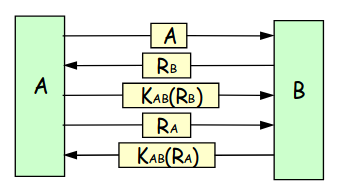
\includegraphics[width=0.4\linewidth]{./images/reto-respuesta.png}
    \label{fig:reto-respuesta}
\end{figure}

Este sistema tiene algunas vulnerabilidades:
\begin{itemize}
    \item \textbf{Ataque por repetición:} el atacante escucha por mucho tiempo y va guardando las respuestas, hasta que se repita un reto y así puede responder. \textbf{Solución:} que el reto no se pueda repetir (NONCE), Ej: fecha + hora. 
    \item \textbf{Ataque por reflexión:} el atacante antes de responder manda el mismo reto, espera a la respuesta y la reenvía. \textbf{Solución:} usar dominios de claves disjuntas.
\end{itemize}

\subsection{Intercambio de Diffie-Hellman}
Permite establecer una clave secreta entre dos entidades a través de un canal no seguro. 
\begin{figure}[H]
    \centering
    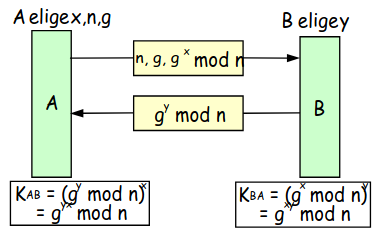
\includegraphics[width=0.4\linewidth]{./images/diffie-hellman.png}
    \label{fig:diffie-hellman}
\end{figure}

\noindent
Este sistema es vulnerable al ataque man-in-the-middle:\\
El atacante se pone en medio e intercepta el mensaje de A, y le manda su propia clave a B, y esa misma clave se la responde a A, y espera que B le responda. De esta forma, hace de mensajero invisible, A y B ni siquiera saben que están escuchando sus mensajes. 

\section{Funciones Hash}

Son funciones de forma que dada una palabra P, nos da una palabra a modo de resumen o compendio de los datos, R. P puede ser de cualquier longitud, R, sin embargo, suele ser de longitud fija y ademas la función es unidireccional, irreversible, es decir, no se puede obtener P a partir de R. Dado un mensaje P, se envía P junto con su hash. \\

Para que no se pueda modificar el mensaje a P' e incluir su resumen se tienen varias alternativas: 
\begin{itemize}
    \item En el resumen podemos meter la clave que se comparte. A este hash (P + $K_{AB}$) se le suele llamar MAC (Message Authentification Code).
    \item Cifrar el hash con la clave compartida.
\end{itemize}

Así conseguimos integridad del mensaje y por otra parte autenticación con los MAC\@.

\subsubsection{MD5 (Message Digest)}

Dada una palabra nos da un resumen de 128 bits. El algoritmo trabaja sobre bloques de 512 bits, por lo que si la palabra no tiene un número de bits múltiplo de 512 rellenamos con 100\ldots0 hasta que sea congruente con 448módulo 512, y se le añade un campo de longitud de 64 bits. A continuación se divide el mensaje en bloques de 512 bits y hacemos un procesamiento secuencial por bloques, es decir, que cada salida sirve como entrada para la siguiente caja MD5\@.


\subsubsection{SHA (Secure Hash Algorithm)}

Funciona igual que MD5 pero los resúmenes son de 160 bits. 


\section{Firma digital y certificados digitales}

Una \textbf{firma digital} intenta ser un sustituto de una firma escrita para poder garantizar el \textbf{no repudio} en nuestras acciones en Internet. Con ellas conseguimos:
\begin{itemize}
    \item Autenticación por parte del receptor de la identidad del emisor.
    \item No repudio por parte del firmante.
    \item El emisor obtiene garantía de no falsificación. (Integridad).
\end{itemize}

\subsection{Firma con clave secreta o Big Brother (BB)}

El protocolo consiste en usar una entidad en la que todos los usuarios confían y que vigilará las transacciones de todos los usuarios. Es una especie de man-in-the-middle. Si A quiere enviar un mensaje a B, el BB formará parte de la comunicación haciendo de puente que guardará cada una de las transacciones realizadas. 

\begin{figure}[H]
    \centering
    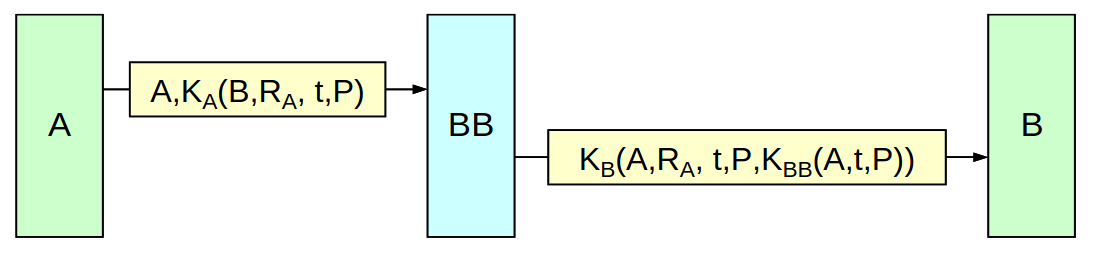
\includegraphics[width=0.8\linewidth]{./images/big-brother.png}
    \label{fig:big-brother}
\end{figure}

El BB tiene una clave compartida con todos. A le manda a BB:
\begin{description}
    \item [A:]Identificador.
    \item [B:] El destinatario.
    \item [$R_A$:] Un resumen para dar integridad.
    \item [t:] el instante de tiempo.
    \item [P:] texto plano, el mensaje a enviar. 
\end{description}
Todo menos el identificador va cifrado con la clave que comparte A con BB. El mensaje es recibido y reenviado por BB añadiéndole algunos detalles.
\begin{description}
    \item [$K_{BB}(A,t,P)$:] Esta clave solo la tiene el BB lo que prueba ante un juez quién ha hecho dicha transacción, en qué momento y el contenido de la transacción.  
    \item [$K_B(\ldots)$:] Además todo va cifrado con la clave de B para confidencialidad. 
\end{description}


\subsection{Firma digital con clave asimétrica o Doble cifrado}

Supongamos que A le quiere mandar un mensaje a B. La idea se basa en lo siguiente:
\begin{itemize}
    \item $k_{pri_A}\equiv$ autenticación, solo A ha podido cifrarlo.
    \item $k_{pub_B}\equiv$ confidencialidad, solo B podrá descifrarlo.
\end{itemize}
De esta manera, juntando las dos obtenemos autenticación + confidencialidad: $k_{pub_B}(K_{pri_A} (P))$ (puede cifrarse al revés, no es relevante).\\

Sin embargo todo esto no garantiza el \textbf{no repudio}, puesto que nada nos garantiza que A sea el dueño de la clave. Para garantizarlo necesitamos los certificados digitales que deben ser emitidos por autoridades de certificación, que son entidades fiables. 

\begin{definicion}[Autoridades de certificación (AC\@)]
    Entidad que garantiza la asociación entre identidad y claves.
\end{definicion}

\subsubsection{Certificado digital}
El usuario obtiene sus claves pública y privada, envía una solicitud, firmada digitalmente, a la AC indicando su identidad y clave pública. La AC comprueba la firma y emite el certificado: este tiene los datos que a continuación detallaremos y va firmado digitalmente por la clave firmada de la AC con objeto de que el certificado no pueda falseficarse. Campos de un certificado X\@.509:
\begin{itemize}
    \item Identidad del usuario.
    \item Su clave pública.
    \item La AC que lo ha emitido.
    \item Periodo de validez.
    \item Algunos datos más como la versión del certificado, el número de serie\ldots
\end{itemize}

\section{Protocolos seguros}
La seguridad se divide en dos tipos:
\begin{itemize}
    \item \textbf{Perimetral:} uso de \textit{firewalls}, \textit{sistemas de detección de intrusiones} o \textit{sistemas de respuesta}.
    \item \textbf{Seguridad en protocolos:} consiste en usar protocolos para garantizar seguridad.
        \begin{itemize}
            \item Capa de aplicación: PGP o SSH\@.
            \item Capa de sesión (entre aplicación y transporte): TLS\@, SSL\@.
            \item Capa de red: IPSec\@.
        \end{itemize}
\end{itemize}

\subsection{PGP (Pretty Good Privacy)}

Es un protocolo de correo electrónico seguro. 

\begin{figure}[H]
    \centering
    \begin{subfigure}[b]{0.45\linewidth}
        \centering
        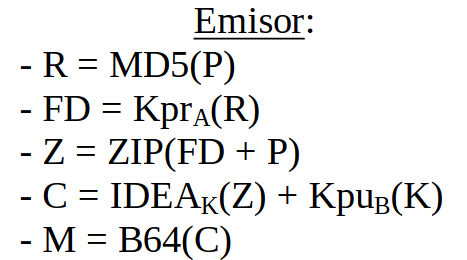
\includegraphics[width=0.6\linewidth]{./images/pgp-emisor.png}
        \label{fig:pgp-emisor}
    \end{subfigure}
    \hfill
    \begin{subfigure}[b]{0.45\linewidth}
        \centering
        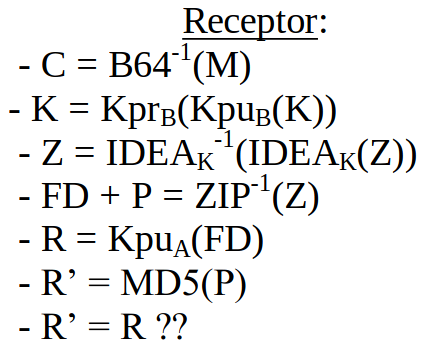
\includegraphics[width=0.6\linewidth]{./images/pgp-receptor.png}
        \label{fig:pgp-receptor}
    \end{subfigure}
\end{figure}

El emisor hace un resumen del mensaje, lo firma; esto lo comprime junto con el mensaje, cifra esa compresión con IDEA y una clave de sesión K (generada solo para esa sesión), que manda cifrada con la clave pública del receptor y esto lo codifica con base 64 (esto no tiene nada que ver con seguridad). El resultado de esto último es lo que le manda al destinatario. El receptor simplemente tiene que hacer el proceso inverso para sacar el mensaje y con el resumen comprobar que no se ha modificado.\\

Con este proceso conseguimos:
\begin{itemize}
    \item Confidencialidad: el mensaje va cifrado.
    \item Integridad: gracias al resumen.
    \item Autenticación: gracias al cifrado con la clave privada.
    \item No repudio: solo si hay un certificado digital.
\end{itemize}


\subsection{TLS\@, SSL}
Se usan para muchos protocolos (HHTPS\@, IMAPS\@, SSL\@-POP\@). TLS fue el original y SSL se acabó popularizando más. Hacen más o menos lo mismo, pero no son compatibles. Lo que hacen en esencia es crear túneles cifrados. 

\subsubsection{SSL}
No es un protocolo sino una familia de ellos.
\begin{itemize}
    \item SSL Record Protocol: encapsula los protocolos y ofrece un canal seguro con privacidad, autenticación e integridad. Lo que se hace es que cuando voy a mandar datos, los parto en fragmentos, cada fragmento lo comprimos, hago un resumen y cifro datos + resumen. Y esto último es lo que se transmite, encapsulado en un paquete TCP\@.
    \item SSL Handshake Protocol: se negocia el algoritmo de cifrado, la función hash, autentica al servidor, el cliente genera claves de sesión (temporales) con el algoritmo de Diffie-Hellman o aleatorias y que irán cifradas con la clave pública del servidor. \\
        El problema del hombre en medio se resuelve autenticando al servidor. Así, si el mensaje que me llega con $g^ymodn$ no viene del servidor no lo tomo. 
    \item SSL Assert Protocol: informa sobre errores en la sesión.
    \item Change Cipher Spec Protocol: para notificar cambios en el cifrado.
\end{itemize}

\subsection{IPSec}
Su objetivo es garantizar autenticación, integridad y opcionalmente privacidad a nivel IP\@. Crea túneles unidireccionales. 

\begin{definicion}[Túnel]
    Es un sitio donde entra un paquete y a la salida tendremos exactamente el mismo paquete. Para ello encapsulamos el paquete dentro de otro paquete. Si el túnel va cifrado (la parte de los datos va cifrada) entonces el túnel es seguro.
\end{definicion}

Son tres procedimientos:
\begin{enumerate}
    \item Establecimiento de una ``Asociación de seguridad'': con el objetivo de establecer una clave secreta (Diffie-Hellman), con la previa autenticación. Es simplex. Vulnera el carácter NO orientado a conexión. 
    \item Garantizar la autenticación e integridad de los datos mediante las ``Cabeceras de autenticación''.
    \item (Opcional) Garantizar la privacidad de los datos mediante el protocolo de ``Encapsulado de seguridad de la carga''.
\end{enumerate}

Dos tipos de túneles:
\begin{itemize}
    \item Modo transporte: la asociación se hace extremo a extremo entre el host origen y destino.
    \item Modo túnel: la asociación se hace entre dos routers intermediarios. Útil por ejemplo si una empresa quiere comunicar dos sucursales, en vez de comunicar cada dos trabajadores, se comunican mediante esos routers intermediarios y solo hacen falta dos túneles (para ambas direcciones).
\end{itemize}


